\documentclass[a4paper,10pt,captions=tableheading,DIV=14]{scrartcl}
\pdfoutput=1

% ----------------------------------------------------------- Packages
\usepackage{amsmath,amssymb,url,cite,slashed,cancel,booktabs,hyperref,graphicx,xspace,subcaption}
\usepackage{braket}
\usepackage[capitalize]{cleveref}
%%%UNUSED%%% \usepackage{feynmp,enumerate,multirow,wrapfig}
\renewcommand\citepunct{,\penalty1000\hskip.13emplus.1emminus.1em\relax} % no line-break in \cite
\renewcommand\thefootnote{*\arabic{footnote}}
\numberwithin{equation}{section}
% COMMENTS
\newcommand{\comment}[1]{{\textbf{\small \color{red} [#1]}}}
\newcommand{\cmark}{\ding{51}} % check mark
\newcommand{\xmark}{\ding{55}} % X mark

% MATH NOTATION
\newcommand\w[1]{_{\mathrm{#1}}}
\newcommand\vc[1]{{\boldsymbol{#1}}}
\newcommand\dd{\mathop{}\!\mathrm{d}}
\newcommand\DD{\mathop{}\!\mathrm{D}}
\newcommand\ee{\mathop{}\!\mathrm{e}}
\newcommand\abs[1]{\lvert#1\rvert}
\newcommand\norm[1]{\lVert#1\rVert}
\newcommand\Abs[1]{\left\lvert#1\right\rvert}
\newcommand\Norm[1]{\left\lVert#1\right\rVert}
\newcommand\ii{\mathrm{i}}
\newcommand\co[1]{\mathrm{c}_{#1}}
\newcommand\si[1]{\mathrm{s}_{#1}}
\newcommand\coco[1]{\mathrm{c}^2_{#1}}
\newcommand\sisi[1]{\mathrm{s}^2_{#1}}
\newcommand\pmat[1]{\begin{pmatrix}#1\end{pmatrix}}
\DeclareMathOperator{\Order}{\mathcal{O}}
\DeclareMathOperator{\sign}{\mathrm{sign}}
\DeclareMathOperator{\ddelta}{\delta}
\DeclareMathOperator{\Tr}{\mathrm{Tr}}
\DeclareMathOperator{\diag}{\mathrm{diag}}
\renewcommand{\Re}{\mathop{\mathrm{Re}}}
\renewcommand{\Im}{\mathop{\mathrm{Im}}}

\newcommand\oneone{1}
\newcommand{\dn}[3]{\frac{\dd^#1 #2}{\dd #3^#1}}    % derivatives
\newcommand{\pdn}[3]{\frac{\partial^#1 #2}{\partial #3^#1}}
\newcommand{\pd}[2]{\frac{\partial #1}{\partial #2}}
\newcommand\parenfrac[3]{\def\temp{#3}\Bigl(\frac{#1}{#2}\Bigr)\ifx\oneone\temp\relax\relax\else^{#3}\fi}
\newcommand\vev[1]{\langle#1\rangle}
\newcommand{\mean}[1]{\left\langle #1 \right\rangle}

\newcommand\hc{\text{h.c.}}

% units
\newcommand\unit[1]{\,\mathrm{#1}\xspace}
\newcommand\eV{\unit{eV}}
\newcommand\keV{\unit{keV}}
\newcommand\MeV{\unit{MeV}}
\newcommand\GeV{\unit{GeV}}
\newcommand\TeV{\unit{TeV}}
\newcommand\PeV{\unit{PeV}}
\newcommand\fb{\unit{fb}}
\newcommand\pb{\unit{pb}}
\newcommand\iab{\unit{ab^{-1}}}
\newcommand\ifb{\unit{fb^{-1}}}
\newcommand\ipb{\unit{pb^{-1}}}
\newcommand\fm{\unit{fm}}


% scientific form of numbers
\makeatletter
\def\EE{\@ifnextchar-{\@@EE}{\@EE}}
\def\@EE#1{\ifnum#1=1 \times\!10 \else \times\!10^{#1}\fi}
\def\@@EE#1#2{\times\!10^{-#2}}
\makeatother

% ---------------------------------------------------- For Sho's Notes
\usepackage{scrlayer-scrpage,color,soul}
\usepackage[hhmmss]{datetime}
\newdateformat{mydate}{\THEDAY\;\shortmonthname.\;\THEYEAR}
\addtokomafont{pagehead}{\small\normalfont}
\ohead{\texttt{[\jobname~@~\mydate\today~\currenttime]}}
\bibliographystyle{utphys27mod}

% --- minted experimental
\usepackage{ifplatform,listings}
\lstset{columns=[l]fullflexible,basicstyle=\small\ttfamily,xleftmargin=2em,frame=L,keepspaces=true}
\ifshellescape
\usepackage{minted}
\setminted{linenos,xleftmargin=7\fboxsep,breaklines,fontsize=\small,frame=leftline,stepnumber=5,framesep=2\fboxsep,escapeinside=||,mathescape=true}
\setminted[console]{xleftmargin=6\fboxsep,frame=none}
\else
\makeatletter
\lstnewenvironment{minted}[1]
  {\csname\@lst @SetFirstNumber\endcsname}
  {\csname\@lst @SaveFirstNumber\endcsname}
\makeatother
\fi
% ---

\newcommand{\mathfunc}[2]{\mathcmd{#1}\texttt{[}\matharg{#2}\texttt{]}}
\newcommand{\mathcmd}[1]{\textup{\texttt{#1}}}
\newcommand{\mathtext}[1]{\textup{\texttt{"#1"}}}
\newcommand{\matharg}[1]{\textsl{#1}}

\newcommand{\TODO}[1]{{\textbf{\lstset{}\color{red}$\clubsuit$#1}}}

% commands for this document
\definecolor{navy}{rgb}{0,0,0.5}
\newcommand\Damu{\Delta a_\mu}
\newcommand\amu[1][\relax]{\ifx#1\relax{a_\mu}\else{a_\mu^{\mathrm{#1}}}\fi}
\newcommand\smu{\tilde\mu}
\newcommand\smuL{\tilde\mu\w L}
\newcommand\smuR{\tilde\mu\w R}
\newcommand\lL{\tilde l\w L}
\newcommand\lR{\tilde l\w R}
\newcommand\neut  [1][\relax]{{\tilde\chi^0_{#1}}}
\newcommand\charP [1][\relax]{{\tilde\chi^+_{#1}}}
\newcommand\charM [1][\relax]{{\tilde\chi^-_{#1}}}
\newcommand\charPM[1][\relax]{{\tilde\chi^\pm_{#1}}}
\newcommand\file[1]{\lstinline[basicstyle=\ttfamily\color{navy}]{#1}}
\newcommand\package[2][\relax]{\texttt{#2}\ifx#1\relax\relax\else~\texttt{#1}\fi}

\newcommand{\gL}{g\w L}
\newcommand{\gR}{g\w R}
\newcommand{\PL}{P\w L}
\newcommand{\PR}{P\w R}

\newcommand{\thuz}{\tilde h\w u^0}
\newcommand{\thdz}{\tilde h\w d^0}
\newcommand{\thup}{\tilde h\w u^+}
\newcommand{\thdm}{\tilde h\w d^-}

\author{Sho Iwamoto}
\title{Details of each benchmark line}
\begin{document}
%\maketitle
\begin{center}{\makeatletter
{\huge\usekomafont{title}\@title}\par\vspace{2em}
{\Large \@author}\par\vspace{2em}
}
\begin{abstract}\noindent
Details (fail safe note) for each of my analyses.
\end{abstract}
\end{center}
\begin{align*}
\lL &= (\tilde e\w L, \tilde \mu\w L, \tilde\tau\w L),
&
\tilde\nu &= (\tilde \nu_e, \tilde\nu_\mu, \tilde\nu_\tau),
&
\text{slepton}=(\lL,\tilde\nu, (\lR)),
\\
l&=(e,\mu,\tau),
&
\ell&=(e,\mu),\dots
\end{align*}

%---------------------------------------------------------------------
\section{Decay chain categorization}

\begin{align}
 \text{chain-3L}&: \neut\charP\to(\lL \nu;\text{1/3 each})+(\lL^{(*)}l^{(*)} \text{ or }\tilde\nu^{(*)}\tilde\nu^{(*)}\text{; 1/12 each}) \otimes(\lL\to l\neut[\text{LSP}], \tilde \nu\to\nu\neut[\text{LSP}]; \text{100\%})
\end{align}
ATLAS 1803 analyzes Chain 3L by ``a statistical combination of the five SR3-slep regions.'' The SRs require three signal lepton ($\ell$)\footnote{Note that they do not define ``signal tau.''}, where the lepton $\ell$ may as well come from leptonic tau decays.


\section{tab1-0.50}

\begin{figure}[h]
  \centering
  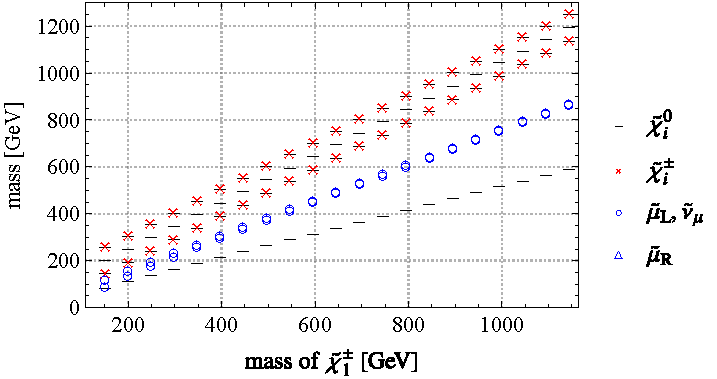
\includegraphics[height=125pt]{../plots/plot_data_tab1_x050.pdf}
  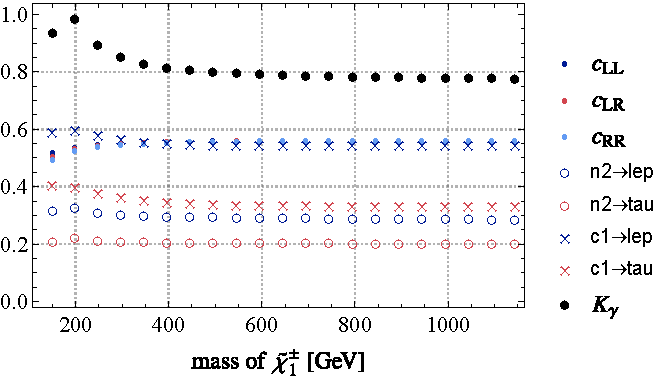
\includegraphics[height=125pt]{../plots/plot_data_tab1_x050_cfactors.pdf}
  \caption{Mass spectrum and $c$-factors of tab1-0.50 benchmark line. The models are generated with $M_2=200,250,\dots,1200\GeV$, while $m_{\charPM[1]}$ is used to label.}
\end{figure}

This line is characterized by
\begin{equation}
 M_2=\mu=2M_1,
\quad
 x = \frac{m_{\tilde l\w L}-m_{\neut[1]}}{m_{\neut[2]}-m_{\neut[1]}}=0.5,
\quad
 \tan\beta=40,
\quad
 \tilde l\w R, \tilde q, \text{heavy-Higgs: decoupled}.
\end{equation}
The mass spectrum is shown below, and we use $m_{\charPM[1]}$ (in GeV) as the label of each model point.

P$<$300 is not considered in our analysis, as neither by ATLAS. P150 has $\tilde\nu$-LSP.

In P$\ge$300, $\neut[2]\charPM[1]$ mainly produces chain-3L.
Also, $\neut[3,4]$ and $\charPM[2]$ decays similarly.
We safely ignore $\neut[3]$ because of non-degeneracy and, as it has less $\tilde W$-component, smaller production rate.
A degenerate pair $\neut[4]\charPM[2]$ may serve as the chain-3L target.
At this first stage I will ignore it, but it may be interesting to include the effect (but how?).

The $c$-factors are similar and thus we use the factor
\begin{equation}
 K_\sigma = \mathop{\mathrm{mean}}(c\w{LL},c\w{LR},c\w{RR})
\end{equation}
to compensate the difference in production cross section from pure-wino (ATLAS 1803) case.
We thus estimate the production cross section as
\begin{equation}
 \sigma(pp\to\neut[2]\charPM[1])\approx K\w{sigma}\cdot \sigma(pp\to\tilde W^\pm\tilde W^3),
\end{equation}
where the pure-wino production cross section $\sigma(pp\to\tilde W^\pm\tilde W^3)$ is taken from LHCSUSYXSWG\footnote{\url{https://twiki.cern.ch/twiki/bin/view/LHCPhysics/SUSYCrossSections13TeVn2x1wino}}.


The decays of $\neut[2]\charPM[1]$ does not equally branch because of Yukawas and slepton mass differences;
\begin{align}
 \neut[2]:&\quad\tau > e = \mu \gtrsim \nu_e = \nu_\mu=\nu_\tau ~~\text{(also to $Z$, $H$)},
\\
 \charPM[1]:&\quad\tau > e = \mu \gtrsim \nu_\tau\gtrsim \nu_e=\nu_\mu ~~\text{(also to $W^\pm$)}.
\end{align}
In ATLAS analysis, since the $\neut[2]\charPM[1]$ pair is pure-Wino and sleptons masses are degenerate, three-$\ell$ signature is expected by a probability of
\begin{equation}
 \left(\frac23+\frac13p(\ell|\tau)\right)
 \left(\frac4{12}+\frac{2}{12}p(\ell|\tau)\right)\approx0.307,
\end{equation}
where $p(\ell|\tau)\simeq0.352$ is the leptonic decay rate of $\tau$.
We therefore compensate the difference in the branching ratios with $K_\Gamma$-factor:
\begin{equation}
 K_\Gamma = \frac{1}{0.307}
\left[
 p(\tilde\ell\w L,\tilde\nu_\ell|\charPM[1])
+ p(\ell|\tau)p(\tilde\tau\w L,\tilde\nu_\tau|\charPM[1])
\right]
\left[
 p(\tilde\ell\w L^{(*)}|\neut[2])
+ p(\ell|\tau)p(\tilde\tau\w L^{(*)}|\neut[2])
\right]
\end{equation}
(the notation $p(\text{daughters}|\text{mothers})$ should be understood).
Here one should note that we ignore the kinematics difference due to the origin of lepton (whether $\tau$, $\tilde\chi$, or sleptons) as well as slepton non-degeneracy.

We then compare our cross section with $\sigma\w{UL}$; the points with
\begin{equation}
 \frac{K_\sigma K_\Gamma\cdot \sigma(pp\to\tilde W^\pm\tilde W^3)}{\sigma\w{UL}} \ge 1
\end{equation}
are excluded.\footnote{
ATLAS 1803: \url{https://doi.org/10.17182/hepdata.81996.v1/t80}
}
\begin{figure}[h]
  \centering
  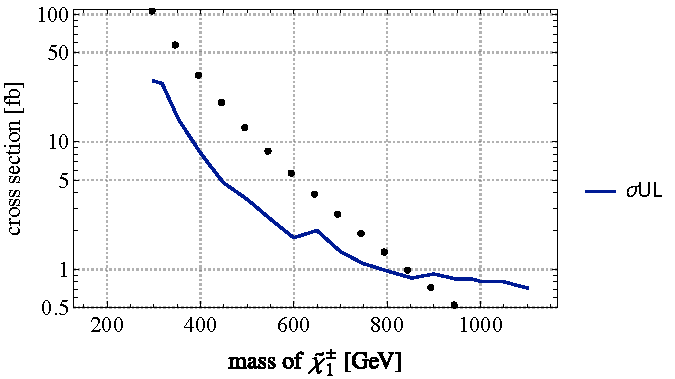
\includegraphics[height=125pt]{../plots/plot_data_tab1_x050_atlas1803.pdf}
  \caption{\label{fig:tab1_x050_atlas1803}ATLAS 1803 analysis (3l-slep) on tab1-0.50 benchmark line.}
\end{figure}

The results against ATLAS1803 is shown in \cref{fig:tab1_x050_atlas1803}, where the black dots correspond to $K_\sigma K_\Gamma \sigma(\text{Wino})$.
It shows that the ATLAS 1803 analysis nearly excludes P900 (and below).
The wiggles in $\sigma\w{UL}$ is due to interpolation of the $\sigma\w{UL}$-grid ATLAS provides, for which logarithmic interpolation (i.e., linear interpolation on the function $\log\sigma\w{UL}(m_{\charPM[1]},m_{\neut[1]})$) is used.




\bibliography{analysis}
\end{document}
